Unfortunately we weren't able to get a MOT which lasted longer than a few seconds. This was due to the error signal for locking the cooling laser. The error signal had a frequency bias such that the desired frequency lied outside the linear part. Therefore there was no efficient feedback and the laser could easily jump to another frequency and we were effectively working with a non locked laser. We wanted to adjust the error signal, but this was denied by the tutor.

So in all following measurements we weren't able to do a full series of measurements with one MOT but rather created a new MOT every time. Errors will be calculated by Gaussian error propagation.

\subsection{Measured data}

Lense diameter: $\si{(38 \pm 3)\, \milli\meter}$

Distance between lense and MOT: $\si{(260 \pm 10)\,\milli\meter}$

Cooling beam power: $\si{(1.2 \pm 0.1)\,mW}$ per axis

Total beam power: $\si{(3.15 \pm 0.01)\,mW}$ per axis

\subsection{Beam size}

\begin{figure}
\centering
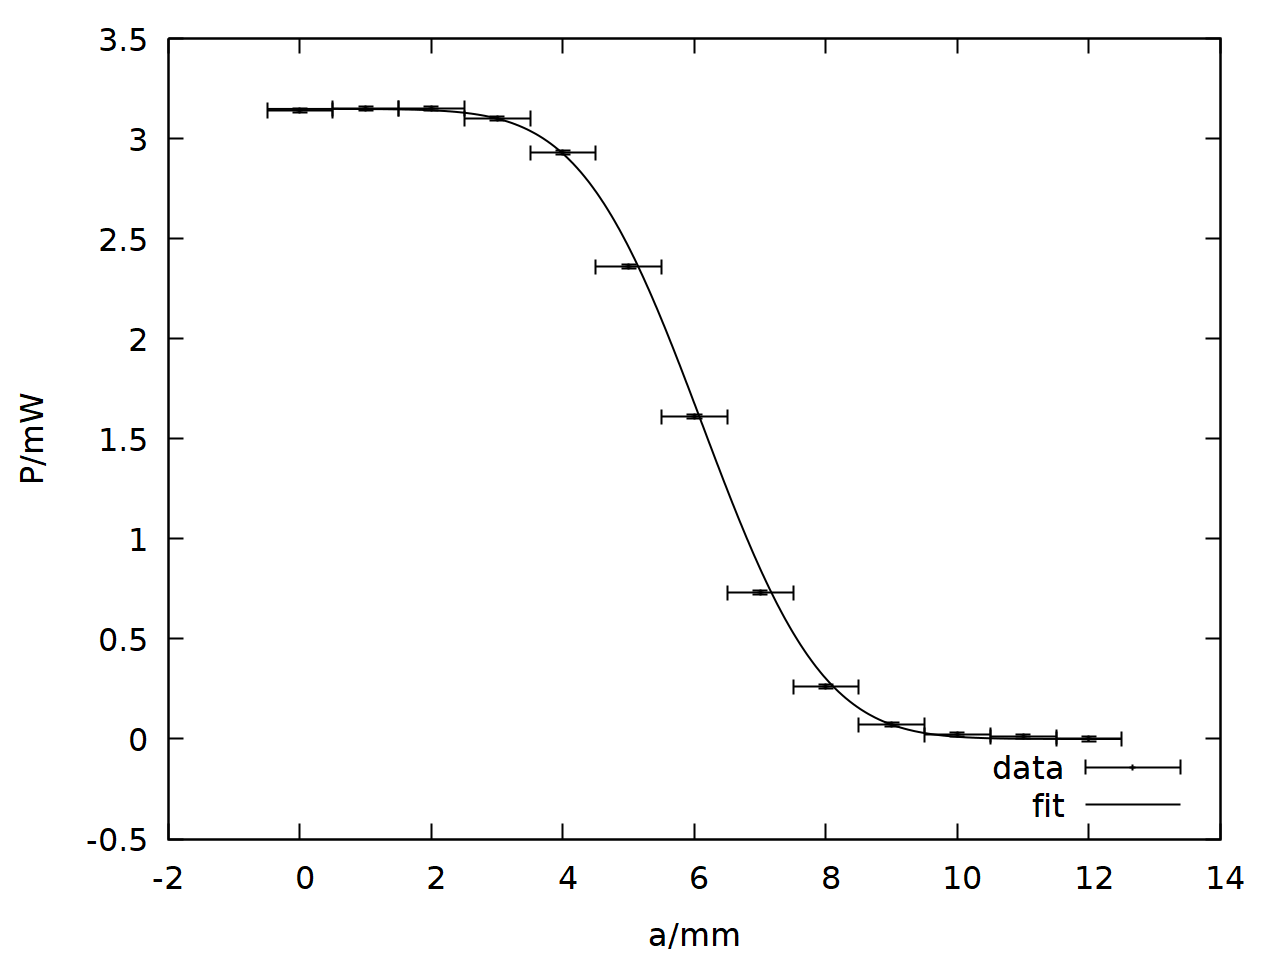
\includegraphics[width=0.7\textwidth]{data/beam.png}
\caption{Beam power over razor blade position and fit}
\label{fig:beam}
\end{figure}

The beam power is plotted over the position $a$ of the razor blade in figure \ref{fig:beam}. Since we assume a Gaussian beam the power is given by the error function, precisely $P(a) = A\qty(1-\erf(\frac{a-B}{\sqrt{2}\sigma}))$. Fitting this function to the data results in $A = \si{(1.574 \pm 0.002) mW}, B = \si{(6.12 \pm 0.09) mm}, \sigma = \si{(1.45 \pm 0.06) mm}$. The $1/e^2$ radius is then given by $4 \sigma = \si{(5.8 \pm 0.2) mm}$.

\subsection{Size of MOT}
In figure \ref{fig:mot} the MOT has dimensions $58\si{px} \times 23\si{px}$. 

\begin{figure}
\centering
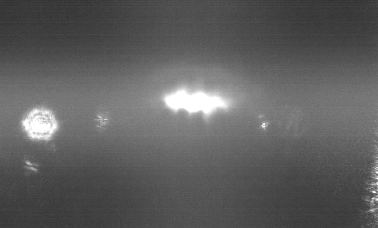
\includegraphics[width=0.7\textwidth]{figures/P102018/mot_2.png}
\caption{Picture of the MOT}
\label{fig:mot}
\end{figure}

Figure \ref{fig:karton} was taken with the same camera settings. The "Bayer Makrolon" measures $\si{(21.5 \pm 0.5) \milli\meter}$ in reality and $575 \si{px}$on the foto.

\begin{figure}
\centering
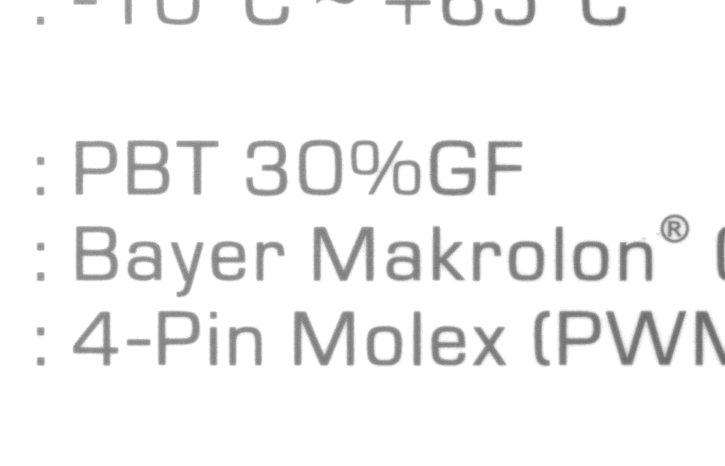
\includegraphics[width=0.7\textwidth]{figures/P102018/karton.png}
\caption{Picture of some text}
\label{fig:karton}
\end{figure}

Using this gauge one can compute the dimensions of the MOT: $\si{(2.2 \pm 0.5) \milli\meter \times (0.86 \pm 0.02) \milli\meter}$. Unfortunately we don't have information about the size of the MOT in z-direction.
